

\chapter{Herstellung und Zusammenbau}
\label{chap:herstllung}

\section{Herstellungsprozess der Komponenten}
\subsection{Skelett und grundlegende Bootsform}
Da für dieses Projekt keine Computergesteuerte \ac{cnc} Fräse zur Verfügung steht werden die Spanten des Bootes mittels einer elektrischen Stichsäge ausgeschnitten. Dafür werden die Baupläne der einzelnen Elemente mithilfe eines Plotters im Massstab 1:1 ausgedruckt und  mithilfe von Backpapier mittels der Abpausmethode auf Tannenholzbretter übertragen, und anschliessend ausgesägt. Dieser Prozess wird in zwei Arbeitsschritte unterteilt. Im ersten Durchgang wird die äussere Form ausgesägt. In einem zweiten Durchgang wird dann Material von innerhalb der Elementen entfernt. Dies wird aus Gewichtsgründen gemacht und schaftt mehr Freiraum im Inneren des Bootes.
An den entsprechenden Stellen an der Oberseite der Elemente werden Löcher gebohrt und die Elemente werden dann mithilfe zweier Aluminiumstangen ineinander befestigt. Um eine Verschiebung der Elemente während des Herstellungsprozess zu vermeiden wird Heisskleber verwendet. 
\begin{figure}[H]
    \centering
    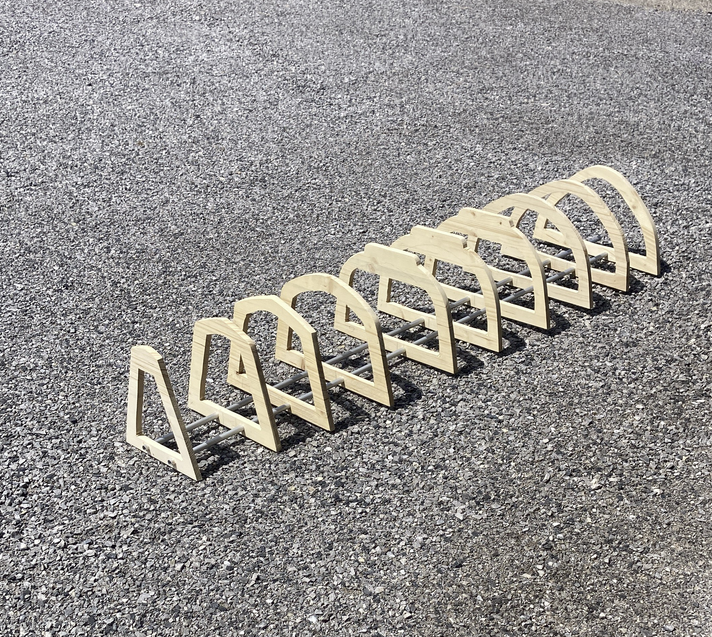
\includegraphics[width=1\linewidth]{rippe1.png}
    \caption{Rippen förmige Anordnung der Tragelemente}
    \label{fig:enter-label}
\end{figure}

Da, wie angetönt, dieser Teil hauptsächlich von Hand gemacht wird, lassen sich  Ungenauigkeiten nicht völlig vermeiden. Diese sind entweder bereits bei der Übertragung des Plans auf die Holzbretter entstanden oder anschliessen beim Aussägen. Daher weichen die tatsächlichen Masse bis zu 5 mm von den Planwerten ab. Dies ist eine sehr hohe Abweichung, die jedoch in den folgenden Arbeitsschritten ausgebessert werden. \\ 
Da für die Elemente aus Kostengründen kein Massivholz genommen werden kann, muss auf Leimholz zurück gegriffen werden. Dies hat zum Nachteil, dass einzelne Elemente einen Bruch erleiden, wenn zu viel Druck auf die geleimten Stellen wirkt. Beschädigte Elemente wurden nicht verwendet und neue wurden Hergestellt. 
\begin{figure}[H]
    \centering
    \includegraphics[width=0.25\linewidth]{bruch.png}
    \caption{Bruch eines Elements}
    \label{fig:bruch}
\end{figure}

Im Anschluss wird eine Schicht Balsaholz über die Rippen gelegt. Dieses hat eine Stärke von 1mm und ist 100cm lang. Zur Befestigung wird eine Tackerpistole verwendet. Durch Verspannungen im Holz gibt es ungünstigerweise gewisse Verformungen, welche sich auf die Schlussendliche Bootsform auswirken kann.

\subsection{Glasfaserbeschichtung}
Um eine strukturell tragende Hülle für das Boot zu schaffen, werden Glasfasermatten verwedet. In Verbindung mit Epoxidharz werden diese unglaublich stabil und sind der goldene Standard im Bootsbau. \\
Es wird sich entschieden, die Matten über eine Holzstruktur zu legen. Dies führt dazu, dass diese die Form des Bootes Annehmen. Das unterliegende Balsaholz ist die Formgebende- und die Glasfasermatten sind Strukturgebende Komponente \\
Dies führt jedoch auch zu Problemen, da es in der Struktur des Balsaholz zu verspannungen kommt und durch eine wechselnder Feuchtigkeitsgrad in der Werkstatt weitere Verzerrungen zu stande kommen, welche sich dann ebenfalls in das Holz Übertragen lassen. Um diese auszugleichen, muss sehr viel Expoxidspachtemasse aufgetragen wird. Dafür wird eine Mischung von Expoixid und entsprechendem Härtungsmittel vorbereitet werden. Dazu werden Microballons dazu gegeben, welche das spätere abschleifen vereinfachen und mit dem zugegebenenen Tixotropiermittel wird eine Dickflüssigkeit erreicht. Dieser Prozess benötigt viele Iterationen, da immer gewartet werden muss, bis die unterliegende Form vollständig ausgetroknet ist.  wobei primär Versucht wird einen möglichst Stromlinienförmigen Körper zu formen.

Da es beim Bug eine Asymetrie gibt, wird an dieser Stelle extra viel aufgetragen. Damit 

\subsection{Ruder}
Das Ruder wurde ebenfalls aus Tannen-Leimholz gesägt welches ebenfalls aus dem \ac{cad} Model entnommen wird. Dieses wird mit dem selben Verfahren, welches bereits für die Elemente angewandt wird, gearbeitet. Mit einem Schliff an der zum Boot gerichteten Seite wird eine verbesserte Hydrodynamik erhofft. Da dies jedoch, wie bereits erwähnt, kein zentraler Punkt der Arbeit ist, werden dafür keine weiteren Analysen oder Simulationen durchgeführt.

\subsection{Kiel}


Hier Bild


\subsection{Segel}
\subsubsection*{Schneidtechnik}
Das Segel besteht aus EPS Platten, welche passend ausgeschnitten werden müssen, um eine möglichts aerodynamische Form zu erhalten. Da konventionelle EPS Schneidgeräte nicht genügend gross sind, muss eine andere Lösung entwickelt werden.  \\
Schneidegeräte dieser Art funktionieren so, dass ein heisser Draht (60$^\circ$ C - 100$^\circ$ C) das EPS zum schmelzen bringt und somit ein sauberer Schnitt entsteht. Der Draht wird durch das Prinzip des Elektrischen Wiederstand erhitzt. Der Draht ist so konstruiert, dass er einen möglichst hohen Wiederstand hat. \\
Das selbe Prinzip wird für dieses Projekt angewendet jedoch modifiziert. Verwendet wird ein Ersatzschneidedraht, ein sogenannter "Wiederstandsdraht" für eine solche Maschine mit einem Durchmesser von $\varnothing$ 0.2mm und einem Labornetzteil welches 12V und max. 3A lifert.
Im ersten versuch wird eine Holzkonstruktion gebaut, welche genug Breit für die EPS Platten ist. Diese besteht aus einem 1.5m langen Balken und zwei senkrecht darauf montieren Halterungen an welchen der Draht befestigt ist. Dieser ist auf einer halb eingeschraubten Schraube aufgerollt und lässt sich durch weiteres Einschrauben, spannen. 


\begin{figure}[H]
    \centering
    \includegraphics[width=0.25\linewidth]{foamcutter1.png}
    \caption{Foamcutter}
    \label{fig:enter-label}
\end{figure}



Es wird jedoch bemerkbar, dass der Draht die Platten nicht durchschneidet. Beim näheren zusammenrücken der Kontakten ist das Durchscneiden jedoch möglich. Daraus kann man vermuten, dass der Wiederstand zwischen den beiden Kontakten zu gross relativ zu der zur Verfügung gestellten Leistung ist. 
Um das Problem zu lösen wird der Durchmesser des drahtes verdoppelt. Dafür werden zwei ursprünglich Drähte ineinander verdreht. Nach einem ersten Test ist es jedoch weiterhin nicht möglich, die Platten wie gewünscht zu durchtrennen. Daher wird ein anderes Netzteil verwendet, welches 21V und max. 5A bereitstellt. Nach diesen Änderungen lässt sich das EPS schneiden. 

\subsubsection*{Grosssegel}
Um die geplante Form aus dem \ac{eps} schneiden zu können, wird diese zuerst die genwünschte Form mithilfe eines Lasercutters erstellt. Diese gilt als Vorlage, welche auf den beiden kürzeren Seiten mit einer Schraube montiert wird. Somit lässt sich der Draht entlang dieser Kante ziehen und die Form wird so ausgeschnitten. \\


\begin{figure}[H]
    \centering
    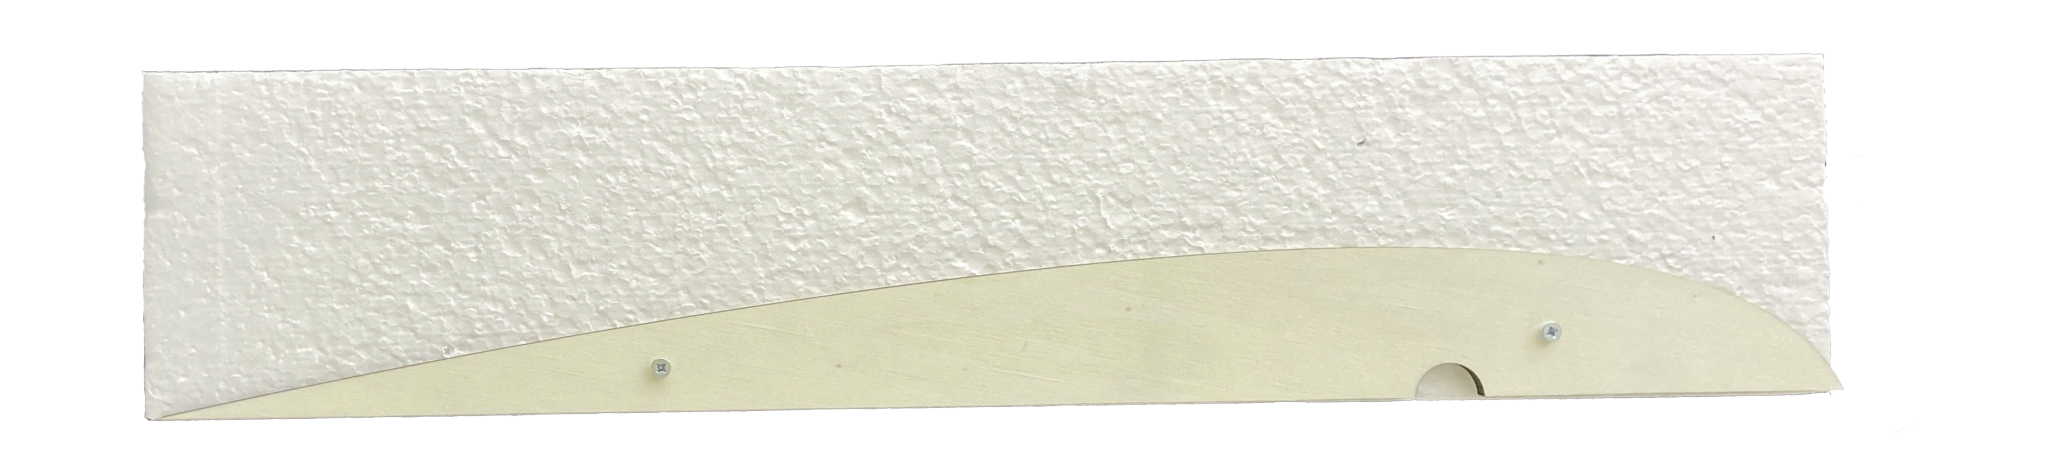
\includegraphics[width=1\linewidth]{assets/template_on_foam.png}
    \caption{Seitenansicht eines Elements mit der Schablone}
    \label{fig:enter-label}
\end{figure}

Aufgrund von kleinen Einkärbungen im Holz oder Ungenauigkeiten beim schneiden, entstehen Unschönheiten im Segel. Diese können entweder durch einen erneuten Durchgang oder durch Schleifen entfernt werden.
\subsection{Saailflap}



\section{Bemalung}
Da das Segelboot gesehen werden sollte, wurde sich für Rot als Signalfarbe entschieden. Diese wurde dann als Seidenmatten Acryllack auf das Boot mithilfe einer Farbwalze aufgetragen. Die Matte Farbe wurde gewählt um ungenauigkeiten in der Bootsform zu verstecken. 

Auch Schutzfunktion bei Ruder, Kiel und Deck

\section{Einbau der Elektronik}
Als erstes wird ein digitaler Schaltplan mit allen Sensoren und Aktuatoren und Sensoren erstellt. Dieser gilt als Bauanleitung für den Bau. Die Informationionen um den Schaltplan herzustellen stammen aus den einzelnen Datenblättern der Sensoren in welchen die Funktions und Betribsweise erläutert ist.

\subsection{Raspberry Pi}
Der Raspberry Pi wird direkt über seinen 5V Pin angesteuert. Vor dem Pi ist ein Downstep Modul plaziert, was den ca. 7V Output der Batterie auf 5V reduziert.
Ein Nachteil bei diesem Ansatz ist, dass der Raspberry die gesamte Schutzelektronik, welche beim USB Port angebracht ist, überspringt. Der Bedeutende Vorteil ist jedoch, dass Verlötete stellen Permanent sind und diese sich ohne erhbeliche Gewalt bei Normaltemperaturen nicht lösen. Bei einem sich durchgehend bewegten System ist dies Notwenig. 
Ein Ausfall der Bordelektronik würde für das Boot katastrophal enden. 


\subsection{Aktuatoren}
Wie im Kapitel "Elektronik" bereits erläutert, verfügen die verwendetet Aktuatoren über 3 pins. V+, GND und einen Datapin. \\
Da der Raspberry pi über seine 5V output pins nicht genügend Leistung für das Betreiben eines, geschweige den mehrerer Aktuatoren, werden diese direkt mit der Batterie verbunden. Über einen "common Ground" kann der Raspberry pi trotzdem den Aktuator ansteuern. Ein weiteres Problem ist jedoch, dass auch der Datapin, der Aufgrund vom geringen Energiebedaf, vom Raspberry pi angesteuert werden kann, nicht auf 5V sonder 3.3V basiert. Daher ist der Aktuator auch hier nicht direkt ansteuerbar.
\\
Um dieses Probelm zulösen muss auf einen Levelshifter zurückgegriffen werden, um den 3.3V output auf 5V hoch zu steppen. 




%% Grafik einfügen